% This is samplepaper.tex, a sample chapter demonstrating the
% LLNCS macro package for Springer Computer Science proceedings;
% Version 2.20 of 2017/10/04
%
\documentclass[runningheads]{llncs}
%
% Hie muss normalerweise nichts angepasst werden
\usepackage{graphicx}
\graphicspath{{img/}}
\DeclareGraphicsExtensions{.pdf,.jpeg,.jpg,.png}
\usepackage[cmex10]{amsmath}
\usepackage{algorithmic}
\usepackage{array}
\usepackage[autostyle=true,german=quotes]{csquotes}
\usepackage{booktabs}
\usepackage{xcolor}
\usepackage{listings}             % Source Code listings
\usepackage[printonlyused]{acronym}
\usepackage{fancyvrb}
\usepackage[no-math]{fontspec}

% Font für Unicode zeichen
\newfontfamily\DejaSans{DejaVu Sans}

% Farben definieren
\definecolor{linkblue}{RGB}{0, 0, 100}
\definecolor{linkblack}{RGB}{0, 0, 0}
\definecolor{darkgreen}{RGB}{14, 144, 102}
\definecolor{darkblue}{RGB}{0,0,168}
\definecolor{darkred}{RGB}{128,0,0}
\definecolor{comment}{RGB}{63, 127, 95}
\definecolor{javadoccomment}{RGB}{63, 95, 191}
\definecolor{keyword}{RGB}{108, 0, 67}
\definecolor{type}{RGB}{0, 0, 0}
\definecolor{method}{RGB}{0, 0, 0}
\definecolor{variable}{RGB}{0, 0, 0}
\definecolor{literal}{RGB}{31,0, 255}
\definecolor{operator}{RGB}{0, 0, 0}
\definecolor{primary}{RGB}{128,0,0}
\definecolor{accent}{RGB}{0,0,168}

\usepackage[ngerman]{betababel}
\usepackage[
      unicode=true,
      hypertexnames=false,
      colorlinks=true,
      colorlinks=false,
      linkcolor=darkblue,
      citecolor=darkblue,
      urlcolor=darkblue
   ]{hyperref}
%	 \PrerenderUnicode{ü}

% Einstellungen für Quelltexte
\lstset{
    xleftmargin=0.1cm,
    basicstyle=\scriptsize\ttfamily,
    keywordstyle=\color{keyword},
    identifierstyle=\color{variable},
    commentstyle=\color{comment},
    stringstyle=\color{literal},
    tabsize=2,
    lineskip={2pt},
    columns=flexible,
    inputencoding=utf8,
    captionpos=b,
    breakautoindent=true,
    breakindent=2em,
    breaklines=true,
    prebreak=,
    postbreak=,
    numbers=none,
    numberstyle=\tiny,
    showspaces=false,      % Keine Leerzeichensymbole
    showtabs=false,        % Keine Tabsymbole
    showstringspaces=false,% Leerzeichen in Strings
    morecomment=[s][\color{javadoccomment}]{/**}{*/},
    literate={Ö}{{\"O}}1 {Ä}{{\"A}}1 {Ü}{{\"U}}1 {ß}{{\ss}}2 {ü}{{\"u}}1 {ä}{{\"a}}1 {ö}{{\"o}}1
}



% Makros für typographisch korrekte Abkürzungen
\newcommand{\zb}[0]{z.\,B.\ }
\newcommand{\dahe}[0]{d.\,h.\ }
\newcommand{\ua}[0]{u.\,a.\ }
\newcommand{\bzw}[0]{b.\,z.\,w.\ }

% Emojis und andere Unicode Sonderzeichen
\newcommand{\checkmark}[0]{\DejaSans ✔}
\newcommand{\cross}[0]{\DejaSans ✖}

% Wo liegt Sourcecode?
\newcommand{\srcloc}{src/}

% Zentrierte Tabellen
\newcolumntype{P}[1]{>{\centering\arraybackslash}p{#1}}
 % Weitere Einstellungen aus einer anderen Datei lesen

% Used for displaying a sample figure. If possible, figure files should
% be included in EPS format.
%
% If you use the hyperref package, please uncomment the following line
% to display URLs in blue roman font according to Springer's eBook style:
% \renewcommand\UrlFont{\color{blue}\rmfamily}

\begin{document}
%
\title{WebGL: 3D-Graphics in the Browser\thanks{Hochschule Mannheim}}
%
%\titlerunning{Abbreviated paper title}
% If the paper title is too long for the running head, you can set
% an abbreviated paper title here
%
\author{Moritz Mundhenke\inst{1} \and
Luca Schilling\inst{1}}
%
\authorrunning{F. Author et al.}
% First names are abbreviated in the running head.
% If there are more than two authors, 'et al.' is used.
%
\institute {Hochschule Mannheim, Paul-Wittsack-Straße 10, 68163 Mannheim, Germany
\email{info@hs-mannheim.de}\\
\url{https://www.hs-mannheim.de/}} 
%
\maketitle              % typeset the header of the contribution
%


\begin{abstract}
The abstract should briefly summarize the contents of the paper in
15--250 words.

\keywords{First keyword  \and Second keyword \and Another keyword.}
\end{abstract}
%
%
%
\section{3D Rendering Grundlagen}
\subsection{3D Koordinaten System}
\subsection{Gittergewebe, Polygone und Eckpunkte}
\subsection{Materialien, Texturen und Lichter}
\subsection{Transformationen und Matrizen}
\subsection{Kamreas, Perspektiven, Ansichtsfenster und Projektionen}
\subsection{Shader}



\section{WebGL}
\subsection{Funktionsweise}
WebGL basiert auf der OpenGL ES (Embedded Systems) API \cite{parisi2012webgl} einer reduzierten Version der OpenGL API \cite{KhronosGLES}. Reduziert bezieht sich in diesem Falle jedoch primär auf das Entfernen von Abwärtskompatibilität (\zb fixed-function pipeline) sowie das Wegfallen von Funktionen die softwareseitig durch einfachere Funktionen ersetzt werden (\zb Kein direktes rendering von Quads) \cite{DiffGLES}. Daher können selbst state-of-the-art Engines wie die Unreal Engine mit geringen Einschränkungen verwendet werden um WebGL Projekte zu realisieren \cite{UnrealHTML5}\cite{UnrealLimits}. \\
Da es sich bei WebGL somit um eine low-level Grafikapi handelt, ist die Entwicklung von Anwendung direkt in WebGL sehr Zeitaufwendig und setzt fortgeschrittenes Know-how in Grafikprogrammierung voraus. Daher gibt es einige Frameworks und Game Engines die durch Abstraktionen die Entwicklung wesentlich erleichtern \cite{parisi2012webgl}. Eine exemplarische Übersicht über diese wird in den folgenden Kapiteln gezeigt. \\
Für die Verwendung von WebGL in einer Website wird ein HTML5 canvas Element als Interface zwischen der \ac{DOM} und WebGL benötigt. Von diesem canvas Element kann dann ein WebGL Kontext erzeugt werden \cite{parisi2012webgl}. Dieser Kontext wird dann als Interface für alle folgenden WebGL Operationen verwendet. Konkret würde eine Anwendung 3D Modelle und Texturen laden \bzw erzeugen, diese in Puffer laden um diese dann mithilfe von Shaderprogrammen auf den Canvas Framebuffer zu rendern. 
\subsection{Vorteile und Nachteile}
Um die Vor- und Nachteile von WebGL zu erläutern, werden wir WebGL mit den Webtechnologien Canvas2D, CSS 3D transform und SVG vergleichen. Durch die grundlegende, im vorrangehenden Kapitel beschriebene Ähnlichkeit von WebGL und nativen Grafikapis, wie OpenGL und DirectX, werden diese nicht weiter verglichen.

\begin{table}[ht]
    \centering
    \begin{tabular}{|P{2.5cm}|P{2.5cm}|P{2.5cm}|P{2.5cm}|P{2.5cm}|}
        \hline
        Eigenschaften & WebGL & Canvas2D & CSS 3D &  SVG \\ \hline
        3D & \checkmark & \cross & \checkmark & \cross \\ \hline
        inline HTML & \cross (Proposed) & \cross & \checkmark & \cross \\ \hline
        CSS  & \cross & \cross & \checkmark & \checkmark \\ \hline
        VR & \checkmark & \cross & \cross & \cross \\ \hline
    \end{tabular}
    \caption{Übersicht Eigenschaften von Webgrafiktechnologien}
    \label{table:CompWebtech}
\end{table}

\subsubsection*{Canvas2D}
und WebGL sind sich in der Art der Einbindung in Websites sehr ähnlich. Beide sind als Context eines Canvas HTML5 Elements verfügbar. Wie der Name vermuten lässt ist Canvas2D jedoch auf hardware beschleunigte 2D Grafiken optimiert (Primitive 3D Grafik ist durch softwareseitige Emulation möglich). Dadurch ist es leichter zu verwenden, da der Programmierer sich nicht um low-level Details kümmern muss, sondern direkt 2D Primitive wie Rechtecke, Linien und Kreise zeichnen kann.
\subsubsection*{CSS3d}
bezeichnet eine Reihe von Erweiterung von CSS die das manipulieren von \ac{DOM} Objekten im dreidimensionalen Raum erlauben. Ein Beispiel hierfür ist auf \url{https://developer.mozilla.org/en-US/docs/Web/CSS/transform-function/translate3d} verfügbar. Da alle 3D Element Teil der \ac{DOM} sind, ist CSS3D nicht für komplexe Anwendung optimiert. Besonders Updates der 3D Szene mit vielen Änderung würden zu großen Performanceproblemen führen. Der Haupteinsatzzweck für CSS3D ist somit das darstellen von regulären, möglicherweise auch komplexen wie etwa ganze (Sub-)Seiten als 3D Objekt. Beispielhaft hierfür ein 3D Würfel aus Youtube Videos \url{https://threejs.org/examples/#css3d_youtube}.
\subsubsection*{\ac{SVG}}
\ac{SVG} wurden ursprünglich als statische vektoralternative für reguläre Bilder verwendet. Durch die Einführung von mächtigerem JavaScript und CSS ist es jedoch heutzutage möglich auch interaktive Grafiken mit SVG darzustellen. Die verbreitete Datenvisualisierungsbibliothek d3.js nutzt zum Beispiel SVG zur Anzeige der Grafiken. SVG verwendet, ähnlich wie CSS3D, \ac{DOM} Elemente zur Objektdefinition. Daher ergeben sich die gleichen Performanceprobleme bei größeren \bzw sehr dynamischen Grafiken. Jedoch ermöglicht die Integration mit der \ac{DOM} nicht nur eine einfachere Programmierung, sondern auch die Nutzung von CSS als mächtiges Gestaltungswerkzeug.
\subsection{Frameworks}
Als Übersicht über die verfügbaren WebGL Frameworks haben wir die zwei beliebtesten Frameworks nach GitHub Stars ausgewählt: three.js (59.9k Stars) und pixi.js (29.2k Stars). Abseits von Grafikanwendung existiert auch eine WegGL beschleunigte Version von Tensorflow, einem bekannten Framework für maschinellem Lernen.
\subsubsection*{three.js} Bei dem mit Abstand beliebtesten Framework handelt es sich um eine Bibliothek die auf 3D Anwendung spezialisiert ist und versucht den Programmierer durch Abstraktionen zu unterstützen ohne jedoch die Möglichkeiten der Technologie einzuschränken. Three.js bietet daher zum Beispiel Hilfsroutinen um 3D-Modell- und Texturdateien direkt zu laden, ohne das der Entwickler sich um das erstellen von Vertex- oder Indexbuffer und deren Drawcalls kümmern muss. Ähnlich können Materialeigenschaften durch Standartklassen \bzw einen in JavaScript verfügbaren Node-basierten Materialbuilder erzeugt werden, ohne das händisch low-level Shadercode geschrieben werden muss. Dieses Node-basierte System ähnelt den Grafischen Materialeditoren in modernen Game Engines, wie \zb Unreal, und Modellierungssoftware, wie \zb Blender. Trotz dieser Abstraktionen erlaubt das Framework trotzdem den Zugriff auf die low-level Komponenten falls dies für den Entwickler erforderlich sein sollte.
\subsubsection*{pixi.js} ist ein Framework das auf beschleunigte 2D Grafik optimiert ist. Daher hat die Bibliothek zusätzlich ein kompatibles Canvas2D Renderbackend für Geräte die kein WebGL unterstützen. Als 2D Framework abstrahiert pixi.js den 3D-Geometrieteil mit Vertexbuffern und Modellen komplett. Die Fokus der Funktionalität besteht im Anzeigen von Bildern. Hierfür stellt das Framework Hilfsmethoden für das erstellen von Spriteanimationen, also das animieren ähnlich eines Zeichentrickfilms, sowie auch komplexer Filter wie Tiefenschärfe und optische Verzerrungen. Obwohl das Framework sehr viele Aspekte von WebGL abstrahiert erlaubt pixi.js trotzdem auch teilweise Zugriff auf low-level Funktionen wie das nutzen von eigenen Shaderprogrammen.
\subsection{Game Engines}
Beide der momentan am weitesten verbreitesten Game Engines \cite{UnityDist}\cite{EngineDist}, Unity und Unreal Engine, erlauben WebGL als Zielplattform. Trotz der weiten Verbreitung dieser Engines konnten wir jedoch keine bekannten Beispiele für die Nutzung dieser Technologie finden. Dies könnte sich auf die relativ große Buildgröße zurückführen lassen. Diese kann sich besonders bei Unreal Engine auf mehr als 100 Megabyte belaufen (ausschließlich für Code). Daher ist es nicht unbedingt überraschend das die meisten Entwickler leichtgewichtigere Lösungen momentan bevorzugen. Beispiele hierfür sind die im vorherigen Kapitel genannten Frameworks sowie die JavaScript Game Engine PlayCanvas, die sich nach eigenen Angaben großer Beliebtheit bei Firmen wie Disney, Samsung und King erfreut.


\section{Anwendungsbereiche}
\label{sec:usecases}
In diesem Abschnitt werden einige der aktuellen Anwendungsbereiche von WebGL vorgestellt.
Zu beachten ist, die Abbildungen sind logischwerweiße wieder nur 2D Bilder und können deshalb nicht die vollen Eindrücke der jeweiligen Seiten wiedergeben, dafür ist ein Besuch der Internetseite nötig.
\subsection{Google Maps}
Eine der wohl bekanntesten Beispiele wo WebGL angewendet wird ist Google Maps.
Hierbei profitiert die in Abbildung~\ref{fig:GoogleMaps} gezeigte Satellitenansicht von der dritten Dimension.
Gebäude können dadurch deutlich realitätsnaher dargestellt werden als auf einer einfachen Karte, auf der man nur die Umrisse sieht.
\begin{figure}
    \centering
    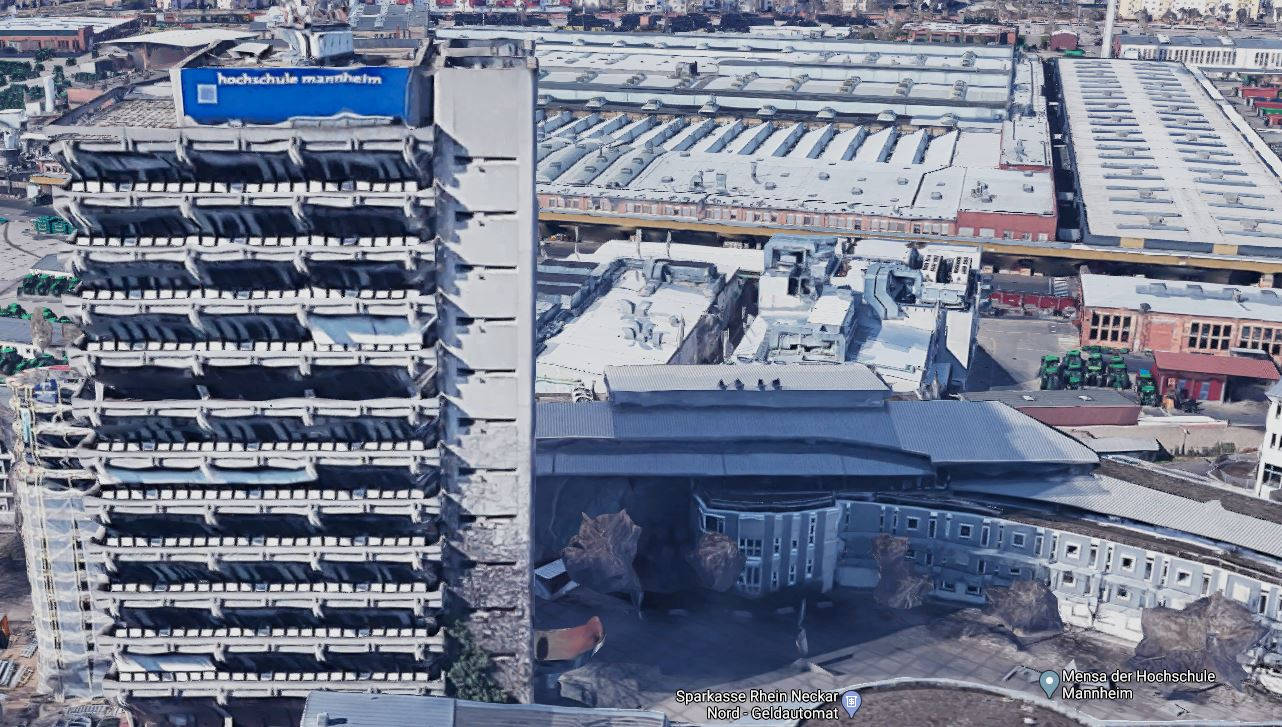
\includegraphics[width=6cm]{GoogleMapsExample.jpg}
    \caption{Google Maps Satellitenansicht \cite{GoogleMaps}} \label{fig:GoogleMaps}
    \end{figure}

\subsection{Online Shopping}
Online Shopping ist ein weiters Beispiel das zur heutigen Zeit fast ausschließlich 2 Dimensional stattfindet.
Durcch die fehlende dritte Dimension können Artikel etwas schlechter angesehen werden, die meisten Online Shopping Seiten versuchen dies durch das Anbieten von Fotos aus verschiedenen Perspektiven zu lösen.
Durch WebGL entsteht die Möglichkeit dies in wirklichem 3D darzustellen, als Beispiel hierfür wurde die Seite Hypebeast gewählt, diese stellt zum Beispiel einen Adidas Schuh auf moderne Art vor, zuerst erhält man eine virtuelle Reise auf der man viele Informationen zu dem besagten Schuh erhält, danach kann man diesen Schuh in 3D anschauen, drehen und die verschiedenen Modelle auswählen was man in Abbildung~\ref{fig:HypeBeast} sehen kann.
\begin{figure}
    \centering
    \includegraphics[width=6cm]{Hypebeast.jpg}
    \caption{Hypebeast Ozweego Presentation \cite{hypbeast}} \label{fig:HypeBeast}
    \end{figure}

\subsection{3D Entwicklung und 3D Druck}
Ein weiterer Bereich in dem WebGL bereits sehr stark angewendet wird, ist die 3D Entwicklung und der 3D Druck. In beiden Bereichen wollen Leute 3D Modelle erstellen und diese an andere Leute Verkaufen.
Damit sich der Käufer die Modelle vor dem Kauf bereits komplett anschauen kann, wird auch hier WebGL verwendet. \cite{manuninja}
In Abbildung~\ref{fig:sketchfab} sieht man ein solches 3D Modell, man kann sich das Modell einfach so anschauen, drehen und vergrößern. Außerdem kann man sich dort auch spezielle Details wie die Knochenstruktur des Modells oder
die verwendete Materialien anschauen. Es ist schon fast genauso gut wie wen man das Modell gekauft und in einem 3D Modellierungsprogramm geöffnet hat. Des weiteren gibt es sogar Seiten die das eigentliche 3D Modellieren im Browser ermöglichen wie zum Beispiel SculptGL. \cite{sculptgl}
\begin{figure}
    \centering
    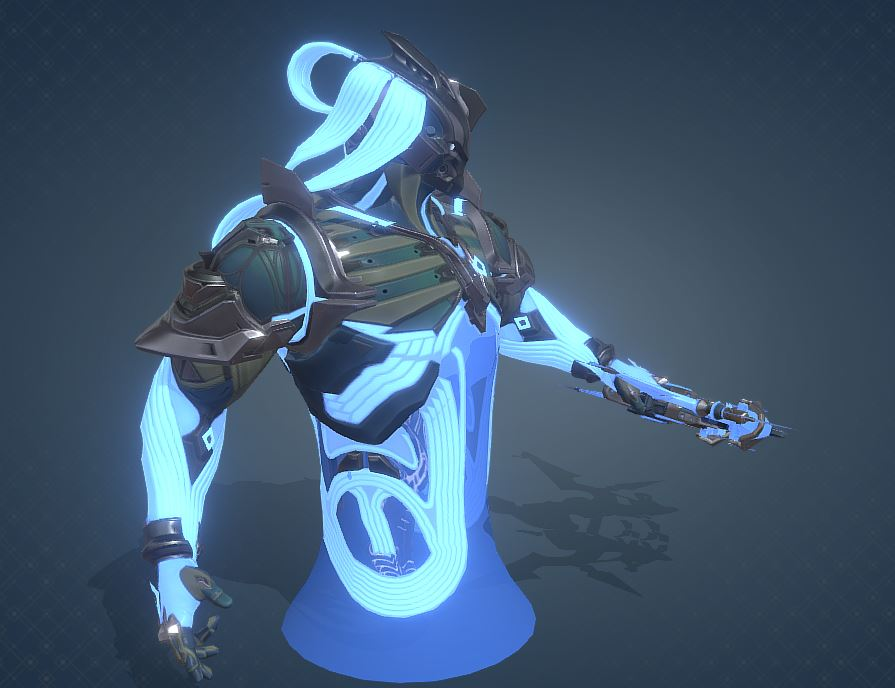
\includegraphics[width=6cm]{sketchfab.jpg}
    \caption{3D Modell Marktplatz \cite{sketchfab}} \label{fig:sketchfab}
    \end{figure}

\subsection{3D Simulationen im Bereich Medizin}
Auch in der Medizin findet WebGL viele Anwendungsbereiche, die Seite BioDigital ermöglicht das Simulieren und Darstellen des Menschlichen Körpers und vielen mehr.
In Abbildung~\ref{fig:BioDigital} sieht man die Simulation eines Menschlichen Körpers der COVID-19 Symptomen aufweißt, diese Simulationen können zur Weiterbildung im Medizinischen Umfeld, zum aufklären von Patienten und vielem mehr verwendet werden.\cite{BioDigital}
\begin{figure}
    \centering
    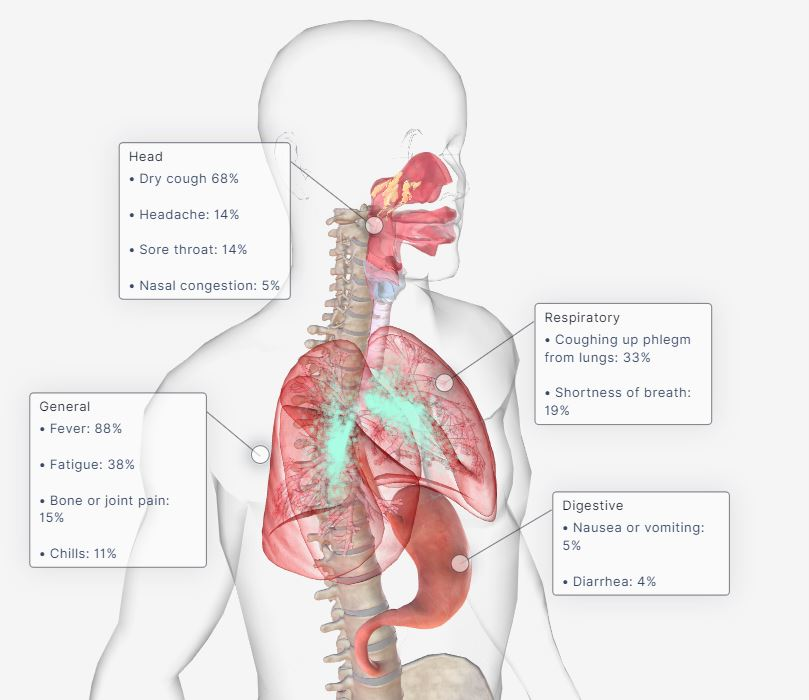
\includegraphics[width=6cm]{BioDigital.jpg}
    \caption{3D Simulation eines Körpers mit COVID-19 Symptomen \cite{BioDigital}} \label{fig:BioDigital}
    \end{figure}

\section{Ausblick}
\subsection{WebGPU}
Bei WebGPU handelt es sich nicht um einen direkten Nachfolger für WebGL, sondern um eine alternative, unabhängige API \cite{WebGPUIntro}. Das auf OpenGL ES basierend WebGL wird daher weiterhin erweitert, momentan auch durch eine größere Neuerung, das auf OpenGL ES 3.0 basierende WebGL2 \cite{WebGL2}. Daher wird WebGPU keine größere Neuerungen in Sachen Funktionalität bieten sondern, ähnlich wie die Vulkan API dem Entwickler genauere Kontrolle über die verfügbaren Ressourcen zu geben und von Grund auf Multithreading zu erlauben. \\
Multi-threading im Web erfordert jedoch weitere neue Technologien da JavaScript im Web ausschließlich in einem Thread laufen kann \cite{JSConcurrency}. Daher wird WebGPU wahrscheinlich häufig oder gar ausschließlich Verwendung zusammen mit Service Workern oder \ac{Wasm} finden, da diese Multithreading erlauben.
Die durch low-level Ansatz von WebGPU möglichen Performancegewinne werden wohl vorallem für Highend Spiele und Computeanwendungen interessant sein. Einfachere Visualisierungen werden womöglich weiterhin WebGL bevorzugen da der zusätzliche Entwicklungsaufwand hier vermutlich nicht die notwendigen Vorteile bringen wird. \\
Zurzeit befinden sich WebGL2 sowie WebGPU noch in experimentellen Stadien.
\subsection{\acf{Wasm}}
JavaScript war für lange Zeit die einzige verfügbare Programmiersprache im offenen Web. Moderne, komplexe Webanwendungen (siehe \ref{sec:usecases} für Beispiele) können jedoch schnell an JavaScripts Performancegrenzen geraten \cite{haas2017bringing}. Um dieses Defizit auszugleichen wurde \ac{Wasm} entwickelt. \ac{Wasm} erlaubt die Ausführung von Programmcode in verschienden Programmiersprachen mit nahezu nativer Geschwindigkeit. Hierfür wird der Programmcode in eine binäre Zwischensprache übersetzt, welche vom Browser geladen und ausgeführt werden kann \cite{WasmMDN}. \ac{Wasm} ist jedoch nicht als Ersatz für JavaScript gedacht. Stattdessen können beide zusammen genutzt werden um die Flexibilität von JavaScript mit der Performance von \ac{Wasm} zu verbinden \cite{WasmMDN}. \\
Obwohl \ac{Wasm} ursprünglich primär für die Nutzung mit low-level Sprachen wie C/C++ entwickelt wurde \cite{WasmMDN}, bieten auch einige high-level Sprachen \ac{Wasm} als Kompiliereziel. Beispiele hier für wären c\# \cite{dotnetWASM} oder AssemblyScript eine auf JavaScript basierend statisch typisierte Sprache\cite{AsmScript}.

%\section{First Section}
\subsection{A Subsection Sample}
Please note that the first paragraph of a section or subsection is
not indented. The first paragraph that follows a table, figure,
equation etc. does not need an indent, either.

Subsequent paragraphs, however, are indented.

\subsubsection{Sample Heading (Third Level)} Only two levels of
headings should be numbered. Lower level headings remain unnumbered;
they are formatted as run-in headings.

\paragraph{Sample Heading (Fourth Level)}
The contribution should contain no more than four levels of
headings. Table~\ref{tab1} gives a summary of all heading levels.

\begin{table}
\caption{Table captions should be placed above the
tables.}\label{tab1}
\begin{tabular}{|l|l|l|}
\hline
Heading level &  Example & Font size and style\\
\hline
Title (centered) &  {\Large\bfseries Lecture Notes} & 14 point, bold\\
1st-level heading &  {\large\bfseries 1 Introduction} & 12 point, bold\\
2nd-level heading & {\bfseries 2.1 Printing Area} & 10 point, bold\\
3rd-level heading & {\bfseries Run-in Heading in Bold.} Text follows & 10 point, bold\\
4th-level heading & {\itshape Lowest Level Heading.} Text follows & 10 point, italic\\
\hline
\end{tabular}
\end{table}


\noindent Displayed equations are centered and set on a separate
line.
\begin{equation}
x + y = z
\end{equation}
Please try to avoid rasterized images for line-art diagrams and
schemas. Whenever possible, use vector graphics instead (see
Fig.~\ref{fig1}).

\begin{figure}
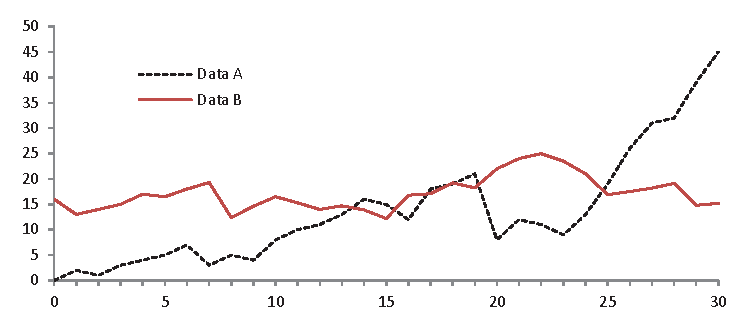
\includegraphics[width=\textwidth]{fig1.eps}
\caption{A figure caption is always placed below the illustration.
Please note that short captions are centered, while long ones are
justified by the macro package automatically.} \label{fig1}
\end{figure}

\begin{theorem}
This is a sample theorem. The run-in heading is set in bold, while
the following text appears in italics. Definitions, lemmas,
propositions, and corollaries are styled the same way.
\end{theorem}
%
% the environments 'definition', 'lemma', 'proposition', 'corollary',
% 'remark', and 'example' are defined in the LLNCS documentclass as well.
%
\begin{proof}
Proofs, examples, and remarks have the initial word in italics,
while the following text appears in normal font.
\end{proof}
For citations of references, we prefer the use of square brackets
and consecutive numbers. Citations using labels or the author/year
convention are also acceptable. The following bibliography provides
a sample reference list with entries for journal Test~\cite{parisi2012webgl} %Comment out if you want to see how some basic stuff should be written with this template


\bibliography{literatur}{}
\bibliographystyle{plain}
\end{document}

